The HEPSPEC ........ allow standardized benchmarking of CPU
performance ......

For an estimate of the performance of the virtual machines, machines
with the same hardware configuration are compared which are either
deployed via the existing Tier2/3 boot system (``bare metal'') or via the NEMO
OpenStack in virtual machines.

The results of the HEPSPEC benchmarks are presented in
Fig.~\ref{fig:HEPSPECpCPUvsCPU-atlas} which shows the HEPSPEC score
determined per number of CPUs versus the number of CPUs.
Different tests have been performed \textit{bare metal}, where the
benchmark code is run either with user rights (``realistic load'') or
with root privileges (``machine reserved'').
The results illustrate that the bare-metal jobs are less performant
than those performed in virtual machines on NEMO with machines under
realistic load. Tests carried out
in user space on the virtual machines are approaching \textit{bare metal} tests with
root permissions.


\begin{figure}[htbp]
%% For example, with the graphicx package use
  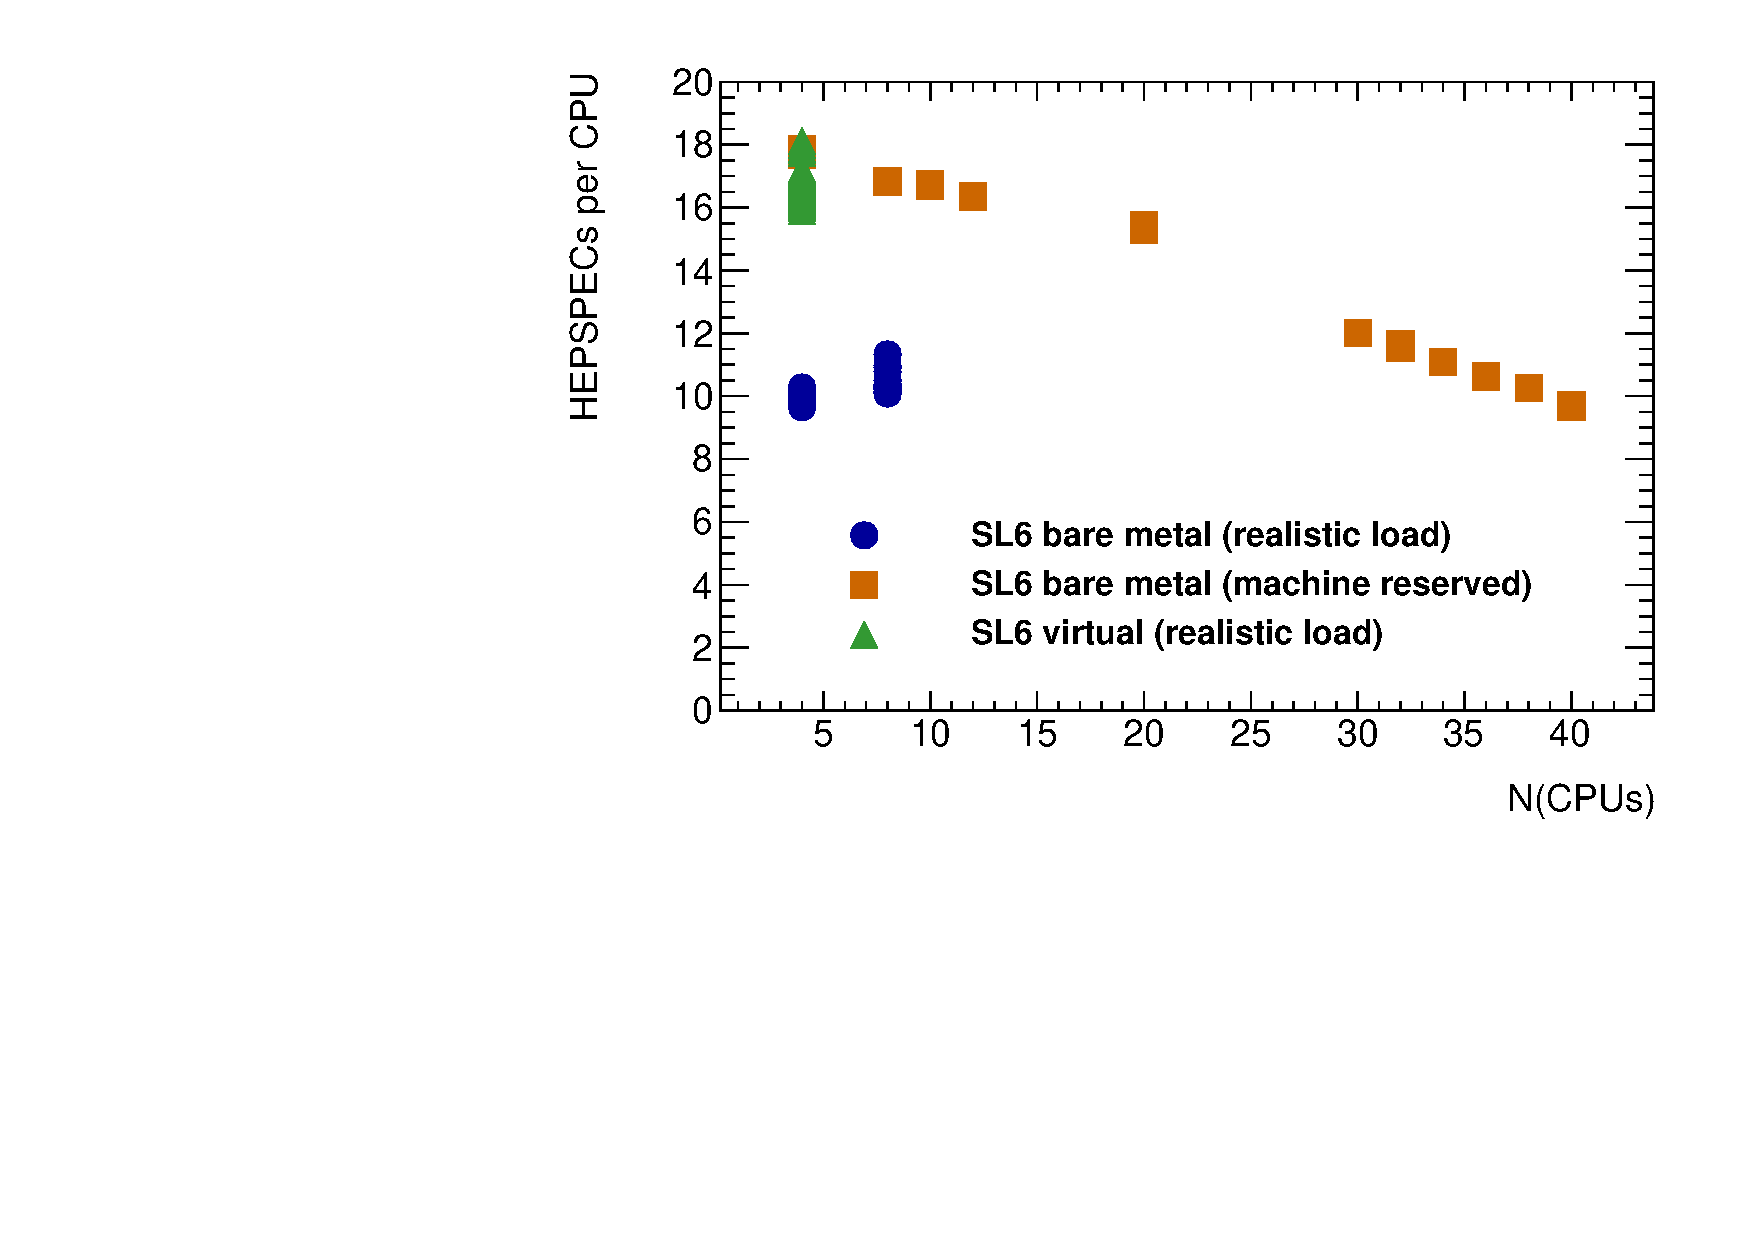
\includegraphics[width=\columnwidth]{figures/HEPSPECpCPUvsCPU.pdf}
\caption{Results of HEPSPEC benchmark tests: HEPSPEC per number of
  CPUs in dependence of number of CPUs.}
\label{fig:HEPSPECpCPUvsCPU-atlas}
\end{figure}

As it is expected from first principles that the virtualisation
reduces the CPU power available to the process, these results indicate
non-optimal configuration of the bare-metal running. However it is
reassuring for the use-case of running in the ATLAS environment on
NEMO that the performance does not suffer.



%
%realistic load: as user
%machine reserved: root
%Hier sieht man, dass die Bare-Metal-User-Jobs wesentlich weniger performant sind, und die User-Jobs auf den VMs beinahe an die ROOT-Tests auf bare-metal herankommen. Interessant ist auch, dass bei den User-Jobs der Trend umgekehrt ist: Dort ist die HEPSPEC pro Core(!) etwas besser fuer 8 Cores. Es koennte aber auch sein, dass das bei den ROOT-Jobs auch so waere, dort haben wir die Zahlen in dem Bereich ja nicht.
%